\documentclass{standalone}

\usepackage[english]{babel}
\usepackage[linesnumbered, ruled, vlined]{algorithm2e}

\usepackage{caption}

% to create listings

\usepackage{listings, lstautogobble}
\lstset{
  autogobble=true,
  frame=single,
}

\lstdefinelanguage{coq}[Objective]{Caml}{
  morekeywords={Structure, Definition, Inductive, list, return},
  sensitive=true
}

% to define font size

\usepackage{ulem}
\usepackage{moresize}
\usepackage{anyfontsize}

% to use tikz and its libraries

\usepackage{tikz-timing}
\usepackage{tikz}

\usetikzlibrary{backgrounds}
\usetikzlibrary{positioning, calc, arrows, shapes, automata, petri, patterns}

% to use tikzmark, to place and refer to marks outside the current figure

\tikzset{every picture/.style={remember picture}}

% styles for transitions

\tikzset{transition/.append style={fill=black!20, thick}}
\tikzset{transition/.append style={fill=black!20, thick}}

% styles for test and inhib arcs.

\tikzstyle{test}=[pre, *-]
\tikzstyle{inhib}=[pre, o-]

% to use colors

\usepackage{xcolor}

%%%%%%%%%%%%%%%%%%%%%%%%%%%%%%%%%%%%%%%%%%%%%%%%%%
%                  BEGIN DOCUMENT                %
%%%%%%%%%%%%%%%%%%%%%%%%%%%%%%%%%%%%%%%%%%%%%%%%%%

\begin{document}

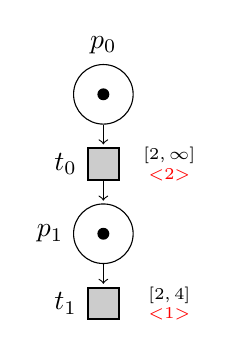
\begin{tikzpicture}
  \node[place, tokens=1] (p0) [label={above:$p_0$}] {};
  \node[place, tokens=1, anchor=north] (p1) at ($(p0.south)-(0,1)$) [label={left:$p_1$}] {};

  \node[transition] (t0) at ($(p0.south)!0.5!(p1.north)$) [label={left:$t_0$}] {}
  edge[pre] (p0)
  edge[post] (p1);
  \node (c0) at ($(t0.east)$) [anchor=west, align=center, text width= 1cm] {
    \ssmall
    $[2, \infty]$
    \textcolor{red}{${<}2{>}$}
    \par
  };
  
  \node[transition] (t1) at ($(p1.south)-(0,.5)$) [label={left:$t_1$}] {}
  edge[pre] (p1);
  \node (c1) at ($(t1.east)$) [anchor=west, align=center, text width= 1cm] {
    \ssmall
    $[2, 4]$
    \textcolor{red}{${<}1{>}$}
    \par
  };
\end{tikzpicture}

\end{document}
%%% Local Variables:
%%% mode: latex
%%% TeX-master: t
%%% End:
